
\chapter{REVISÃO DA LITERATURA} \label{cap:estadodaarte} 


Este texto serve como sugestão para a revisão da literatura de seu trabalho. Aqui terão alguns exemplos de equações, tabelas, figuras e citações. Para citação direta, use o comando ``\textbackslash citeonline$\{label\ da\ ref. \}$'', como por exemplo: \citeonline{simon2006kalman}. Para citações indiretas, use ``\textbackslash cite$\{label\ da\ ref. \}$'', como aqui: \cite{combustaoaplicada}. Cada referência bibliográfica deve ser posta no arquivo "Bibliografia.bib". Neste arquivo contém alguns exemplos para ajudar no preenchimento. O Google Scholar fornece a referência em formato \LaTeX para ser colado neste arquivo, por exemplo.

\section{Equações}

Alguns exemplos de Equações:

%%%%%%%%%%%%%%%%%%%%%%%%%%%%%%%%%%%%%%%%%%%%%%%%%%%%%%%%%%%%%%%%%%%%%%%%%%%%%%%%%%%%%%%%%%%%%%%%%%
Matriz
%------------------------------------------------------------------------------------------------%
\begin{equation}
  f=  \left[\begin{array}{cccc}
         f(0,0) & f(0,1) & \cdots & f(0,N-1)  \\
         f(1,0) & f(1,1) & \cdots & f(1,N-1)  \\
         \vdots & \vdots & \ddots & \vdots \\
         f(M-1,0) & f(M-1,1) & \cdots & f(M-1,N-1)
    \end{array}\right]
\end{equation}
%%%%%%%%%%%%%%%%%%%%%%%%%%%%%%%%%%%%%%%%%%%%%%%%%%%%%%%%%%%%%%%%%%%%%%%%%%%%%%%%%%%%%%%%%%%%%%%%%%

Somatórios
\begin{equation} \label{eq:médiasevarianciasOTSU}
  \begin{array}{rl}
        \mu_1(k)&=\dfrac{1}{P_1}\displaystyle\sum^{k}_{i=0}ip_i= \dfrac{\mu(k)}{P_1(k)} \ ,\\ 
                     \\
        \sigma_1^2(k)&=\dfrac{1}{P_1}\displaystyle\sum^{k}_{i=0}\left[i-\mu_1(k)\right]^2p_i \ ,\\
                     %\sigma_1^2(k)&=\dfrac{1}{P_1}\displaystyle\sum^{k}_{i=0}(\mu_1(k)-p_i)^2\\
                     \\
        \mu_2(k)&=\dfrac{1}{P_2}\displaystyle\sum^{L-1}_{i=k+1}ip_i=\dfrac{\mu_G-\mu(k)}{1-P_1(k)} \ ,\\
                     \\
        \sigma_2^2(k)&=\dfrac{1}{P_2}\displaystyle\sum^{k}_{i=0}\left[i-\mu_2(k)\right]^2p_i \ .\\
    \end{array}
\end{equation}

Equações Alinhadas
%%%%%%%%%%%%%%%%%%%%%%%%%%%%%%%%%%%%%%%%%%%%%%%%%%%%%%%%%%%%%%%%%%%%%%%%%%%
\begin{eqnarray} \label{eq:modelogeralident}
\begin{aligned}
	\noindent 
A(q) \ y(k)&=\dfrac{B(q)}{F(q)}u(k)+\dfrac{C(q)}{D(q)}\nu(k)\\
y(k)&=\dfrac{B(q)}{F(q)A(q)}u(k)+\dfrac{C(q)}{D(q)A(q)}\nu(k)\\
y(k)&=G(q)u(k)+H(q)\nu(k) \ ,
\end{aligned}
\end{eqnarray}
%%%%%%%%%%%%%%%%%%%%%%%%%%%%%%%%%%%%%%%%%%%%%%%%%%%%%%%%%%%%%%%%%%%%%%%%

Outro exemplo:

\begin{eqnarray} \label{eq:polinomiosmodelogeralident}
\begin{aligned}
	\noindent 
A(q)&=1+a_1q^{-1}+\cdots+a_{n_a}q^{-n_a}\ ,\\
B(q)&=b_0+b_1q^{-1}+\cdots+b_{n_b-1}q^{-n_b+1}\ ,\\
C(q)&=1+c_1q^{-1}+\cdots+c_{n_c}q^{-n_c}\ ,\\
D(q)&=1+d_1q^{-1}+\cdots+d_{n_d}q^{-n_d}\ ,\\
F(q)&=1+f_1q^{-1}+\cdots+f_{n_f}q^{-n_f}\ .
\end{aligned}
\end{eqnarray}
%%%%%%%%%%%%%%%%%%%%%%%%%%%%%%%%%%%%%%%%%%%%%%%%%%%%%%%%%%%%%%%%%%%%%%%%%%%%%

Equações Matriciais
%%%%%%%%%%%%%%%%%%%%%%%%%%%%%%%%%%%%%%%%%%%%%%%%%%%%%%%%%%%%%%%%
    \begin{eqnarray} \label{eq:modeloARMAXsisoSS}
        \begin{aligned}
            \centering
                 \begin{bmatrix}
                    x_1(k+1)\\ 
                    x_2(k+1)\\
                    \vdots\\
                    x_{n-1}(k+1)\\ 
                    x_{n}(k+1)
                \end{bmatrix}
                                          =
                \left[\begin{array}{c c c c|}
                  0 & 0 & \cdots & 0 \\
                 \hline
                 1&0 &\cdots &0 \\
                 0&1 &\cdots &0 \\
                 \vdots&\vdots &\ddots &\vdots \\
                 0&0 &\cdots &1 \\
                \end{array}
                %
                \begin{array}{c}
                     -a_n      \\
                      -a_{n-1}      \\
                     \vdots\\
                     -a_2\\
                     -a_1
                \end{array}
                \right]&
                \begin{bmatrix}
                    x_1(k)\\ 
                    x_2(k)\\
                    \vdots\\
                    x_{n-1}(k)\\ 
                    x_n(k)
                \end{bmatrix}
                                            \\&+
                \begin{bmatrix}
                     b_n-a_nb_0\\
                   b_{n-1}-a_{n-1}b_0\\ 
                    \vdots\\
                    b_2-a_2b_0\\ 
                    b_1-a_1b_0
                \end{bmatrix}
                                            u(k)
                                            +
                \begin{bmatrix}
                c_n-a_n\\ 
                c_{n-1}-a_{n-1}\\ 
                \vdots\\% c_{n-p+1}-a_{n-p+1}\\ 
                c_2-a_2\\ 
                c_1-a_1
                \end{bmatrix}
                    \nu(k)
        \end{aligned}
    \end{eqnarray}
    %%%%%%%%%%%%%%%%%%%%%%%%%%%%%%%%%%%%%%%%%%%%%%%%%%%%%%%%%%%%%%
    
    \begin{eqnarray} \label{eq:modeloARMAXsisoSSsaída}
        \begin{aligned}
            \centering
                y(k)
                                          =
                \begin{bmatrix}
                    0   &    0   & \hdots &   0    &  \hdots  &   0    & 1
                \end{bmatrix}
                \begin{bmatrix}
                    x_1(k)\\ 
                    x_2(k)\\
                    \vdots\\
                    x_{n-1}(k)\\ 
                    x_n(k)
                \end{bmatrix}
                                            +
                                                      b_0 u(k)
                                            +
                    \nu(k) \ ,
        \end{aligned}
    \end{eqnarray}
    %%%%%%%%%%%%%%%%%%%%%%%%%%%%%%%%%%%%%%%%%%%%%%%%%%%%%%%%%%%%%%
    
    Outro caso:
    
    %%%%%%%%%%%%%%%%%%%%%%%%%%%%%%%%%%%%%%%%%%%%%%%%%%%%%%%%%%%%%%%%%%%%%%%%%%%%%%%%%%%%%%%
\begin{equation} \label{eq:modeloSSShapingFilter_Estadosaumentado_processo}
     \begin{bmatrix}
        \mathbf{x}(k+1)\\
        \hdashline
        \mathbf{x_f}(k+1)
    \end{bmatrix}
    =
     \left[\begin{tabular}{c:c}
        $A(k)$&$\mathbf{C_f}(k)$\\
        \hdashline
        $\mathbf{0}$&$\mathbf{A_f}(k)$
    \end{tabular} \right]
    %
     \begin{bmatrix}
        \mathbf{x}(k)\\
        \hdashline
        \mathbf{x_f}(k)
    \end{bmatrix}
    +
    \left[\begin{tabular}{c}
        $B(k)$\\
        \hdashline
        $\mathbf{0}$
    \end{tabular} \right] \mathbf{u}(k)
    +
    \left[\begin{tabular}{c}
        $\mathbf{0}$\\
        \hdashline
        $\mathbf{B_f}(k)$
    \end{tabular} \right] \mathbf{w}(k) \ ,
\end{equation}
%%%%%%%%%%%%%%%%%%%%%%%%%%%%%%%%%%%%%%%%%%%%%%%%%%%%%%%%%%%%%%%%%%%%%%%%%%%%%%%%%%%%%%%

\section{Figuras}

%----------------------------------------------------------------------------------------------------%
\begin{figure}[H]%[!htb]
        \centering
      \caption{Exemplo de limiarização de uma imagem de chama a óleo pelo Método de Otsu.}
         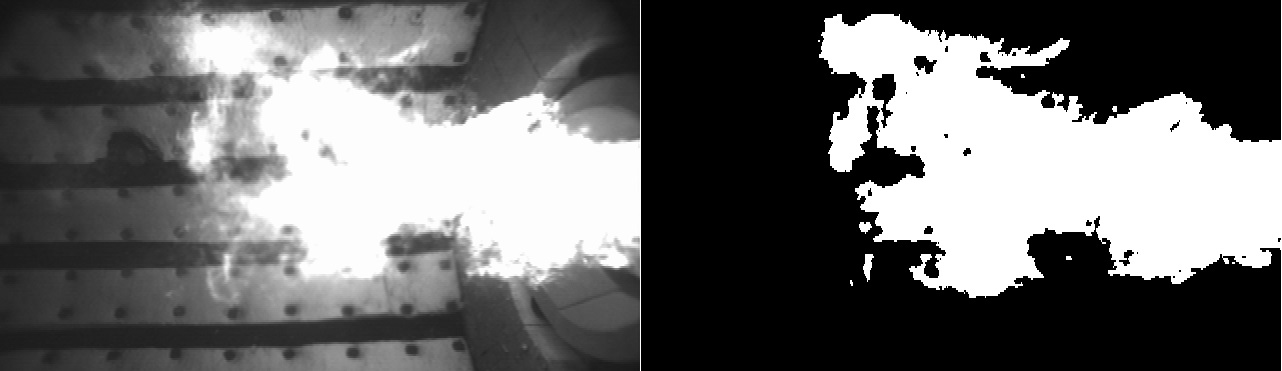
\includegraphics[scale=0.4]{Imagens/OTSU-VVap30kg-0004-impar.jpg}
      %\footnotesize{Fonte: \citeonline{silvaneto-chui2019}.}}
       \label{imagem:limiarizaçãoOTSU}
       \legend{\footnotesize{\citeonline{silvaneto-chui2019}.}}
\end{figure}
%----------------------------------------------------------------------------------------------------%




%---------------------------------------------------------------------------------------------%
\begin{figure*}[h]
\centering
    \subfloat[Painel de Controle]{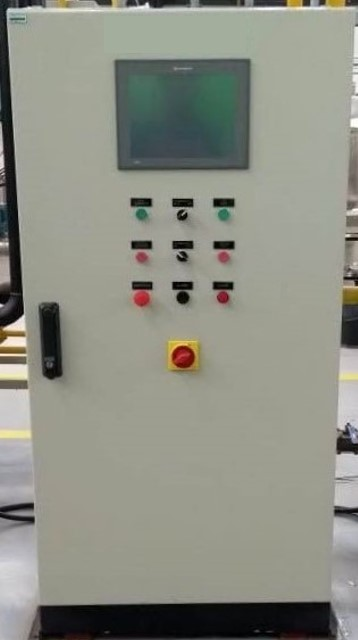
\includegraphics[scale=0.545]{Imagens/painelwhitefisico.jpg}%
    \label{image:caixapainel}}
        \hfil %espaço entre as figuras
    \subfloat[Detalhe da tela sinótica do painel] {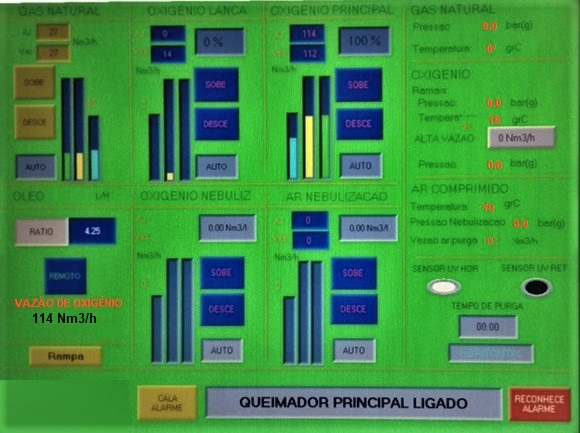
\includegraphics[scale=0.8]{Imagens/painelwhitecopia.jpg}%
    \label{image:telapainel}}
%label da figura toda
\label{image:painel_completo}
%\caption{Painel de controle das vazões de entrada de gás natural e oxigênio puro na fornalha. \footnotesize{Fonte: Elaborado pelo autor.}
\end{figure*}
%---------------------------------------------------------------------------------------------%

\section{Tabelas}

Para as tabelas, existem alguns sites que convertem tabelas em formato .xls e .xlsx em formato \LaTeX. Alguns disponibilizam para você preencher a tabela online, como no site ``https://www.tablesgenerator.com/''. Abaixo, segue um exemplo de tabela simples.

%*************************************************************************%
\begin{table}[htpb]
% increase table row spacing, adjust to taste
\renewcommand{\arraystretch}{1.3}
% if using array.sty, it might be a good idea to tweak the value of
% \extrarowheight as needed to properly center the text within the cells
\caption{Composição química e suas respectivas frações molares e mássicas em base úmida de um determinado gás natural.}
\centering
\begin{tabular}{c c c c}
\hline \hline
Componente & Nome & $\%$f.molar (bu) & $\%$f.mássica (bu)\\
\hline
$CH_4$ & Metano & a & c\\
$C_2H_{6}$ & Etano & b & d\\
$C_3H_{8}$ & Propano & d & e\\
$C_4H_{10}$ & n-Butano & 0,07 & 0,23\\
$C_5H_{12}$ & n-Pentano & 0,01 & 0,04\\
$CO_2$ & Gás Carbônico & 0,48 & 1,19\\
$N_2$  & Nitrogênio & 1,28 & 2,02\\
\hline \hline
\end{tabular}
\label{tab:composicaoquimica}
\\ \vspace{0.1cm}
\legend{\footnotesize{xxx.}}
\end{table}
%*************************************************************************%
\vskip 1cm


